
%%% Local Variables: 
%%% mode: latex
%%% TeX-master: t
%%% End: 

\chapter{相关工作}
\label{cha:relwork}

在现代操作系统研究中,操作系统的多核可扩展性是一个重要研究领域。为了开发多核友好的数据结构和算法,众多研究者已经对Linux内核中的多核优化问题进行了深入研究。例如
MIT PDOS研究组通过修改Linux内自旋锁(spinlock)的API实现\cite{locks:linuxsymp},极大地优化了Linux内核在48核机器上EXIM等应用的性能。下面将对一系列多核优化相关工作进行进一步阐述。

\section{Linux内核多核扩展性研究}
Linux作为服务器系统上应用最广泛的操作系统内核,其多核可扩展性受到广大用户关注。
在学术界和工业界,类Unix操作系统在SMP和NUMA架构上的可扩展性性能研究已经有了很长历史,除了Intel和AMD的多核架构之外,Stanford提出了FLASH研究项目\cite{kuskin1994stanford}、IBM等公司也生产出了几十上百个核的基于共享内存模型的计算机。为了使操作系统在这类硬件上达到良好的可扩展性,可扩展锁、wait-free同步、多核
调度算法、多核内存管理算法等技术被不断提出。这些新技术有的已经在诸如Linux、Solaris等实用操作系统中被广泛应用。

在众多Linux内核研究工作之中,Silas Boyd-Wickizer等人提出了一整套内核可扩展性测试例程Metis\cite{linux:osdi10},发现了Linux中潜在的可扩展性问题并提出了部分解决方案。
在文章中,他们分析了7个重要的系统应用(包括Exim、memcached、Apache、PostgreSQL、gmake、Psearchy和MapReduce)在48核Linux机器上的运行情况。发现除了
gmake之外,所有应用程序都在近期的Linux内核版本中遇到了可扩展性瓶颈。如图\ref{fig:memcached}所示,实验证明,在Linux中随着CPU核数增多,memcached的性能反而下降。

\begin{figure}[ht]
\begin{center}
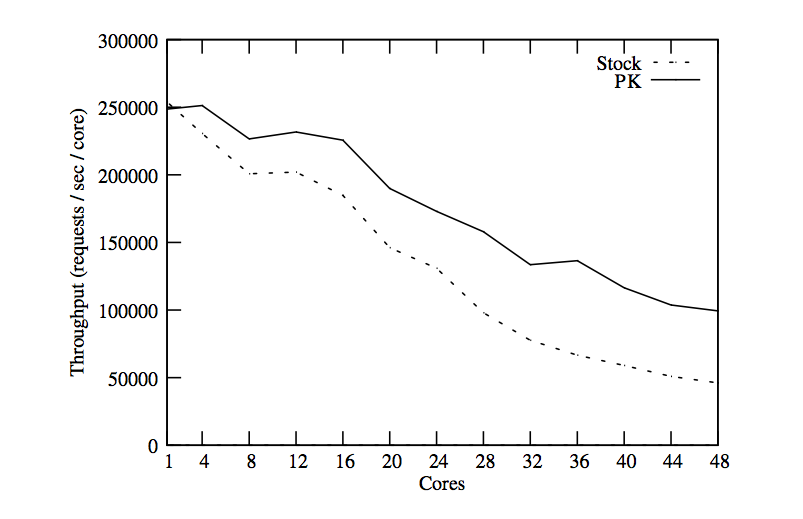
\includegraphics[width=0.7\textwidth]{figures/memcached_test.png}
\end{center}
\caption{memcached吞吐量\cite{linux:osdi10}}
\label{fig:memcached}
\end{figure}

根据已有研究工作造成操作系统扩展性问题的原因总结有:

\begin{itemize}
\item 对共享数据结构加锁,核数增多造成各CPU在核上等待时间变长。
\item 在不同CPU上读写同一内存位置(包括假共享),这会在硬件保证Cache一致性的平台上带来额外的Cache一致性协议开销
\item 多个进程或线程竞争有限的Cache,降低CPU的Cache命中率
\item 多个进程或线程竞争有限的内存带宽
\end{itemize}

从上述几点看以看出,造成操作系统或应用程序在多核平台上性能问题的一个主要原因来自于数据共享,以及为了保护共享数据而
加上的锁。因此,有研究者通过设计新的数据结构管理内核对象,以此减少共享数据带来的开销。此外,文章还总结了10多个造成多核性能瓶颈的关键代码点,
并对Linux做出对于修改。他们修改了Linux2.6.35-rc5,使之在多核平台上性能表现显著提升。

\section{K42实验操作系统}
K42\cite{Krieger:2006:KBC:1218063.1217949}是由IBM公司开发的一个与Linux二进制接口兼容的可扩展操作系统内核。K42在设计之初就考虑到多核硬件上的可扩展性,遵循减少核间数据共享、最大化数据局部性达这一原则。K42的设计者通过以下四项技术优化它的多核可扩展性:
\begin{itemize}
\item 使用客户端-服务器端模型提供系统内核服务。系统服务通过过程调用的方式提供给客户端,客户端的系统服务请求总是有本CPU核上的服务线程处理,避免核间通讯;
\item 感知数据局部性的内存分配器;
\item 面向对象的设计方式。系统服务操作只施加在受影响的对象上,以此限制数据访问的局部性;
\item 使用一个名为Clustered Object的统一模型,对内核对象进行管理。这一编程模型使用分布式系统的方法,提供可扩展的对象冗余(replication)、数据结构和算法划分操作。
\end{itemize}

K42的主要不足是开发时间距今太长,主要面向PowerPC架构,对NUMA系统的支持不够成熟等。

\section{MIT xv6实验操作系统}

在工业界,Linux开发者在不断优化Linux内核对象的数据结构,以求达到在SMP和NUMA系统上达到线性的多核可扩展性能。尽管Linux内核在最新40核以上系统中部分子系统性能表现不佳,但多年来Linux开发者在内核多核性能优化做出的杰出的努力:

\begin{itemize}
\item Linux kernel 2.0引入SMP架构支持;
\item Linux kernel 2.5允许内核抢占(preempt);
\item Linux kernel 2.6.19中引入了当前使用的RCU实现;
\item Linux kernel 2.6.39版本正式移除的内核大锁(Big Kernel
Lock),在此之前大部分Linux的内核态代码不支持同时在多个CPU上运行。
\end{itemize}

但是,Linux在一些重要子系统中还是使用粒度较大的锁来保证内核数据的一致性。最明显的一个子系统就是Linux的虚拟内存管理子系统。mmap和munmap两个系统调用是Linux中使用最频繁的系统调用之一,但是对于每个进程,Linux使用一个大锁来保护其VMA结构体:

\begin{lstlisting}
/* Linux 3.9.2 mm/utils.c */
down_write(&mm->mmap_sem);
ret = do_mmap_pgoff(file, addr, len, prot, flag, pgoff,
		&populate);                        
up_write(&mm->mmap_sem);                               
\end{lstlisting}

如上面代码所示,Linux中对同一进程的mmap调用都加上了锁,实际上串行化了所有虚拟内存分配操作,这成为一些了单进程多线程的应用程序(如Java虚拟机的多线程内存分配器和垃圾回收器)的瓶颈。

为了解决这些问题,学术界提出了各种各样的解决方法,MIT
PDOS研究小组的Austin T. Clements等人提出了多种解决多核操作系统内数据竞争问题的新型数据结构\cite{radixvm:eurosys13}。设计了运行在AMD64平台的操作系统内核xv6。并基于xv6实验OS实现了一个全新的虚拟存储管理模块RadixVM,在80核机器上获得
了几乎线性的加速比。他们主要工作有:
\begin{itemize}
\item 使用Refcache替代传统的原子加减操作
\item 使用改进Radix
Tree实现VMA映射,使得对虚拟地址不重叠的的mmap和munmap操作可以完全并行地进行
\item 跟踪每个CPU内核的内存使用,只对必要的CPU内核进行TLB Shootdown操作
\end{itemize}

相关研究人员在80核的机器上经行了实验,发现RadixVM系统在非重叠虚拟内存区域中达到了完美可扩展。换言之,如果多个线程并行地地经行mmap和munmap系统调用,这些调用可以完全独立运行,并且不会带来Cache一致性协议造成的多核通讯流量。


\section{操作系统接口改进研究}
除了对操作系统内部对象数据结构的改进,也有部分研究把重心放在寻找和优化操作系统对用户程序的接口(主要是系统调用)的优化上。
Baumann等人以此为基础,设计了一个新型的支持异构多核硬件的操作系统Barrelfish\cite{Baumann:2009:MNO:1629575.1629579}。
他们认为,把分布式系统中信息传递(Message-Passing)的思想应用到传统操作系统之中。他们认为当前和未来多核硬件会越来越解决于网络系统,这促使我们用分布式系统的思想重新考虑操作系统的设计。因此,他们抛弃过去的基于共享内存的多核操作系统设计方式,把系统中的进程看做发布系统的节点,在它们之间通过信息传递的方式交换信息。Baumann等人认为,他们的设计的操作系统Barrelfish(图\ref{fig:barrelfish})比起传统操作系统设计,更容易适应未来多核硬件的发展。

\begin{figure}[ht]
\begin{center}
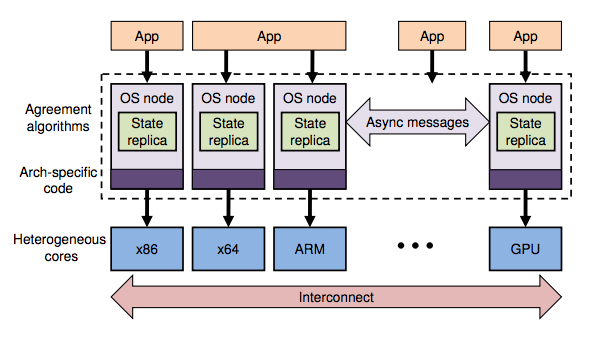
\includegraphics[width=0.7\textwidth]{figures/barrelfish.png}
\end{center}
\caption{Barrelfish系统架构\cite{Baumann:2009:MNO:1629575.1629579}}
\label{fig:barrelfish}
\end{figure}

也有研究者通过通过截然不同的方法来挖掘操作系统接口的并行性。有研究者\cite{commuter:2013}通过对操作系统Posix API建模的方法,求解系统调用的可交换性,从而分析不同调用参数和执行路径形成的共享数据依赖关系并寻找潜在的多核可扩展空间。这种方法将在后面的章节仔细讨论。

综上所述,目前多核操作系统的可扩展性研究仍然是目前研究的热点,各国研究机构和公司都在提出各自的操作系统内核解决方案。因此,在最新的多核硬件上实现一个实验用多核可扩展操作系统内核将为以后的操作系统优化工作打下重要的基础。


